%
% start (TODO: clean up; some bits esp. about Stata are already in the introduction)
%

\chapter{Computers}%
  %
  %
  \label{ch:computers}%
  %
  %
  \index{Computers}%
  %
  %

\begin{quote}%
  Digital technology is programmed. This makes it biased toward those with the capacity to write the code. In a digital age, we must learn how to make the software, or risk becoming the software. It is not too difficult or too late to learn the code behind the things we use—or at least to understand that there \emph{is} code behind their interfaces. Otherwise, we are at the mercy of those who do the programming, the people paying them, or even the technology itself.%
  
  \footcite[128]{Rushkof2010}
\end{quote}

A course on quantitative methods is bound to make intensive use of computer software. You all use computers routinely for many different activities, but your level of familiarity with some of the fundamental aspects of computers can vary dramatically.

Being reasonably familiar with computers is required for this course: please read this section in full and assess whether you are familiar enough with the notions covered. A reasonable level of familiarity with computers will help you with using Stata and completing assignments, and will also generally come in handy.

All instructions assume that you are using a personal laptop to run the course, as we do. The computers available at Sciences Po come with system-wide restrictions that will not allow you to modify your workstation as explained below.

This section covers three topics related to computer use in this course:

\begin{enumerate}
	\item How to set up a workflow on your laptop
	\item How to write code as Stata do-files
	\item How to get help offline and online
\end{enumerate}


% =============
% = INTERNALS =
% =============


%
%
\section{Components}

A lot of the following makes more sense if you sort out what a computer is in the first place. From the standard user's perspective, a computer is (increasingly) just a machine in a family of devices like mobile phones or tablets. From a more informed perspective, which we need to work rather than simply interact with the machine, we need to detail a few specifications.

To check your current level of proficiency, see how much time you need to describe the model, processor and amount of RAM (Random Access Memory) of your computer, as in a  and 8GB of 1066MHz DDR3 RAM.

For example, the principle of file paths is immediately familiar to users who have already used a terminal to access their data, because a terminal lets you access your disk without the graphic user interface and shows you the actual architecture of your system and files.

Let's start with a quick overview of computer components.


%
\paragraph{Hardware and software}%
	\index{Computers!Hardware and software}

Your computer's physical and electronic parts (hardware) include input and output (I/O) devices like your keyboard and screen, a central processing unit (CPU) and memory storage, both as hard drive space and as ``live'' or ``virtual'' random access memory (RAM), which is used to read and write data more rapidly. All components communicate with each other over a communication network called the bus.%

The software of your computer are the programs that you use to send instructions to the hardware layer. Your operating system provides an initial layer of software that you can then expand with additional programs like Stata to perform more specific tasks. The speed at which you are doing all this is determined by the amount of RAM that you have at hand, by the speed at which you can read or write to your hard drive, and by the speed of your processor, the `CPU'.%


%
\paragraph{CPU (Central Processing Unit)}%
	\index{Computers!CPU (Central Processing Unit)}

The CPU performs arithmetic and logic operations on your computer data and stores their intermediate results. It also controls how tasks are executed on your system by allocating them processor time to compute. If you live in the early twenty-first century, there is a fair chance that your laptop runs a multi-core processor with several linked microchips that can compute separate tasks in parallel.%

Your CPU operates at a given cycle speed, which is currently calculated in GigaHertz (GHz). The 2.53GHz Intel Core 2 Duo CPU that ships with the Apple MacBook Pro, for example, is a dual-core processor that ticks at the clock rate of 2.53 billion cycles per second. These cycles are used to process low-level program instructions that underlie the software that you use. That software might live on your computer or in the cloud.%
  \footnote{See, for instance, the OpenCPU project for statistical computing: \url{https://public.opencpu.org/pages/}}%

%
\paragraph{Logic gates and truth tables}%
	\index{Computers!Logic gates}%
	\index{Computers!Truth tables}
	
Your computer is made of digital circuits that implement logic gates, such as the ones shown in Figure~\ref{fig:gates}. These gates provide the basic mathematic logic that is also used in the software layer of your computer, as when you make use of logical statements to manipulate your data in Stata.%
  \footnote{See Table~p.~\ref{tbl:logical-symbols} at p.~\pageref{tbl:logical-symbols}.}%

\begin{figure}[h]
	\begin{circuitikz}
		\draw (0,0) node[american and port,color=s1] (aand) {};
		\draw (2.5,0) node[european and port,color=s2] (eand) {};

		\draw (5,0) node[american or port,color=s1] (aor) {};
		\draw (7.5,0) node[european or port,color=s2] (eor) {};

		\draw (9,0) node[american not port,color=s1] (anot) {};
		\draw (12,0) node[european not port,color=s2] (enot) {};
	\end{circuitikz}

	\caption{The \texttt{AND}, \texttt{OR} and \texttt{NOT} logic gates in American (red) and European (blue) representations.}%
	\label{fig:gates}
\end{figure}

These logic gates allow your computer to understand basic truth tables, as with the union of two conditions \texttt{A AND B}, their intersection \texttt{A OR B}, or the negation of \texttt{A}, \texttt{NOT A}. Combinations of logic gates are then used to build electronic circuits with two stable states, a.k.a. ``flip-flops''. All data in a computer are stored in that form as binary digits.%

%
\paragraph{Bits and bytes}%
%
A \emph{bit} is a single binary digit (0/1). Modern processors use units of data, or ``words'', that go from 8 to 64 bits. A \emph{byte} is a series of eight bits and a ubiquitous standard in computer architecture. Given that a bit take two values, a byte can take $2^8=256$ values to express a number in the $0-255$ range, or to represent up to 256 characters.%

In a computer environment, larger arrays of bits and bytes provide more power to process and define whatever stuff you are dealing with. The current Unicode UTF-8 standard, for instance encodes text in several alphabets by using up to four bytes to define thousands of different characters. The same logic applies to graphics on a video game console.%

The current technological frontier puts your computer processor at either 32-bit or, for the most recent machines, at 64-bit. Stata~12 for Windows is distributed in two versions for this reason. Stata~12 for \OSX natively supports both processors. Using the 64-bit application should provide a bit more speed on intensive tasks with large datasets.%

%
\paragraph{Operating system}%
%
Your operating system (OS) manages your files, I/O devices, memory and networks. It manages each application as a process, uses your hard drive to swap data in and out of virtual memory, and makes multi-tasking possible by switching very quickly between programs. Your OS also comes with a graphical user interface (GUI) that it superimposes on command-line instructions.%

Working with Stata actually requires that you reverse that last operation, and that you do \emph{not} use the graphic user interface of the software but instead learn how to program Stata directly from the command line. This step in turn asks for a more organized computer workflow than you might be used to.%

You have a cardinal imperative to use the command line as soon as you are conducting research that requires to be examinable by others, which is the case in this course and in many research settings. The first step of that process is to make your research \emph{replicable} by bundling the replication material (the code and possibly the data) with your analysis.%

Making your research examinable by others also has implications in terms of \emph{openness}, which might mean making your research public. While this is not required in this course, bear in mind that some past students have used their research project as starting blocks for public documents like \textsc{MSc} dissertations or working papers.%

% ============
% = WORKFLOW =
% ============


%
\section{Workflow}%
	\index{Computers!Workflow}

On a computer, your workflow is determined by how your operating system lets you handle files, folders and applications. Several professions rely on daily computer use that require to develop a work environment made of several software components organized a common file architecture. Have a look at the interviews published at \emph{The Setup} website\footnote{\url{http://usesthis.com/interviews/}} for example workflows by academics, developers and engineers, but also animators, graphic designers and writers.%

Building a full-fledged Stata workflow would take more time than we have on our hands. If you want to have a look at how sophisticated that operation can get, look at the table of contents of J. Scott Long's book \emph{The Workflow of Data Analysis Using Stata}.\footnote{\url{http://www.stata.com/bookstore/workflow-data-analysis-stata/}}. For our purposes, we will aim at something much simpler: making sure that your computer will not get in the way while we work on replicating and writing do-files in Stata.%


%
%
\subsection{System}

There are more or less efficient ways to deal with your workstation, but your first step should always consist in running an up-to-date operating system on reliable hardware with enough memory and disk space to perform basic functions. Therefore, make sure that your laptop is more than barely operable, and perform all necessary system or hardware updates to dispose of a functional workstation.


\paragraph{System memory}%
%
Stata requires a few hundred megabytes (MB) of memory to operate properly, and the course itself requires the same to install on your hard drive. To run Stata without overloading your system, quickly check that your computer runs with at least one gigabyte (GB) of live memory, and that your hard drive has at least 4GB of remaining space for caching and swapping.

Run as little stuff as possible in parallel to Stata if you want to have a chance to focus on what you will be doing with it. Quit idle applications, remove any nagging notification system that destroys your ability to focus, and close the files and windows for which there will be no use during your work session. That will also help your computer memory.

Stata 11 or older will require that you manually allocate it some memory to store datasets. You are spared from that if you are using Stata 12. %% TODO: add ref. to Sec 3 subsec on set mem.


\paragraph{File paths}%
%
Your computer keeps your files at specific locations that you can browse and modify. These locations are called paths. They usually start with an indication of which drive you are using, then continue with a folder hierarchy, and end with a file or folder name. 

Example paths to the \SRQM folder are \texttt{/Users/fr/Documents/Teaching/SRQM/} on my computer, running Mac OS X, and \texttt{C:\textbackslash{}Users\textbackslash{}Ivo\textbackslash{}Desktop\textbackslash{}SRQM} on Ivaylo's computer, running Windows.

For this course, you will need to locate the \SRQM folder on your computer through its path, which is why we recommend that you move it to an easily accessible and permanent location. Use a simple location, like your \texttt{Documents} folder, to avoid losing time on locating files. Most importantly, \textbf{do not modify any element of this path during the semester}, to avoid breaking your setup.

Using your system through file paths will become useful when we later open datasets and do-files from Stata. For the time of this course, you are advised to . Do not modify the names or locations of the folders that lead to it either.


\paragraph{File names}%
%
Filenames are another essential aspect of computer use, especially when you are handling a large number of files and/or using multiple copies of the same file. Some general recommendations apply:

\begin{itemize}
	\item In all cases, filenames should be short and informative. Regularly accessed files, like datasets, have short filenames for faster manipulation, and contain additional information like the time period covered by the data.
	
	\item In some cases, filenames require \textbf{normalization}. This implies using sensible filenames and standard version numbers for files that are chronologically ordered. This point is important because you will be required to normalize the filenames for your work files in this class. %%% TODO: add ref to Part 3.
\end{itemize}


\paragraph{File formats}%
%
Stata reads and writes to particular file formats. The course itself will also require that you can decompress \ZIP files and read documents in Adobe \PDF format. Your operating system should offer native or out-of-the-box support for both: if you are not sure that it does, check by reading your system documentation, and download freeware solutions if needed.


%
%
\subsection{Tips}

Some tricky aspects of your system can make you lose or save a lot of time. Here are three tips that apply to our work.


\paragraph{Launching applications}%
%
You will need to find a way to quickly access Stata. Your system should have some form of `task bar' where it shows open applications and lets you install shortcuts to your most common programs. On Mac OS X, you can keep Stata permanently in the Dock for easier access, or you can search for it in Spotlight to launch it from there.%
  \footnote{There are more sophisticated launchers, like the one I use in class, Alfred (\url{http://www.alfredapp.com/}). Another launcher for Mac OS X is Quicksilver (\url{http://qsapp.com/}), which is free and open-source.}%


\paragraph{Switching windows}%
%
During class, you will often need to switch from an application to another one. On Windows, use \kbd{Tab-Shift} to browse through all opened windows across all applications. On Mac OS X, use \kbd{Cmmd-Tab} to switch applications, and use \kbd{Cmmd-\`{}} (grave accent) to flip through an application's window. This will come in handy as soon as you start working with do-files.%


\paragraph{Downloading files}%
%
When downloading files, do not let your browser use counter-productive settings like downloading files to temporary folders and then automatically opening them. These settings make it painful to go and fetch the actual file and then opening it with relevant software. Always ask your browser to download files to your Desktop or to an identifiable downloads folder, and disable any option to automatically open them.

Some browsers might also add file extensions to your downloads. For instance, if your browser automatically adds a \ext{.txt} extension to your do-files, you will need to rename the file by turning its file extension back to just \ext{.do} to open it correctly in Stata.

Google Chrome, Mozilla Firefox and Apple Safari are common Internet browsers with appropriate ``Save As'' options available from their contextual menus. Figure~\ref{fig:save-as} shows the contextual menu for Google Chrome on Mac OS X.

\begin{figure}
	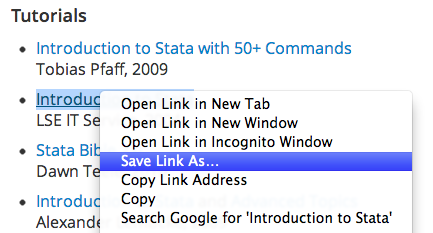
\includegraphics[scale=.5]{images/macosx-save-as.png}
	\caption{The ``Save Link As…'' option in Google Chrome for Mac OS X.}
	\label{fig:save-as}
\end{figure}


\paragraph{External editors}%
%
The scripts that we will use to run Stata commands can be written in any plain text editor. Many of these editors are designed to support a variety of language syntaxes and to let you control visual schemes, code indentation and many other aspects of programming.%
  \footnote{Some free options are TextMate on \OSX (\url{http://macromates.com/}) and Notepad++ on Windows (\url{http://notepad-plus-plus.org/}).}%

For the purpose of this course, you will only need to read and write code from Stata itself. Users who have to deal with longer projects, however, will often develop a workflow organized around a plain text editor that can also be used to write code in other languages. Other professions, like screenwriters, often pick up similar habits with different software.%

For tasks that require working collaboratively over several text documents, developers and programmers also use version control software to share and keep control over large volumes of files. You will not need to use anything like this for this course, but the course itself was developed in such an environment and is available online as a GitHub repository.%
  \footnote{\url{http://github.com/briatte/srqm}}%

%
%
\subsection{Backup}%
%
Avoid data loss purgatory by copying your important files to different locations. Here are three suggestions to keep your personal data safe:%

\paragraph{Files} %
First, set up a backup service like Dropbox or Google Drive, which will seamlessly sync a few gigabytes of data with an online backup server for free. You might also want to consider making regular copies of all relevant files from your hard drive to a USB key or to an external drive.%

\paragraph{Email} %
Next, backup all email correspondence to a personal account, so that you can purge your university email account and avoid maxing it out by exceeding its (limited) capacity. The standard solution for an efficient work mailbox is Google Mail, which can also send and receive larger files.%

\paragraph{Paper} %
Finally, your research paper requires particular attention, as you will need to work as a group on several versions of it. Google Documents is particularly appropriate for collaborative work, but any alternative solution is acceptable, as long as it can contain figures and tables, print to PDF format and properly handle editing from two users or more.%
  \footnote{Most students use either Microsoft Office or Open Office, which are both acceptable, \emph{as long as you actually know how to use the software and backup your work regularly}.}%

All three suggestions above imply that you do not mind putting your precious personal work files in the data cloud hung over our heads by the Google and Dropbox overlords. You will have to trust their shadow armies of engineers buried in pretty dimly lit data centers all over the map. This guide, for example, probably exists at more than four different locations at all times.


% ========
% = CODE =
% ========

%
\section{Code}%
	\index{Computers!Code}%
	\index{Stata!do-files!Syntax}

Stata can execute code written in Stata syntax. Here are three basic code sessions.

%% --------- TODO: add from Sec 2.6.

%
%
\subsection{Running commands}%
	\index{Stata!Commands}

The ‘command line’ terminal works by entering lines of instructions that are reproduced, along with their results, in another window. The next sections of this guide ex-plain further how Stata works and document the usual commands used in this course for data management, description, analysis and graphing. A ‘cheat sheet’ for these commands is offered in Section 12. %% TODO: add ref.

\paragraph{Syntax}%
%
A Stata command is simply a line of code written on a distinct line of a do-file. The Stata do-file editor shows line numbers so that you can easily navigate through long documents.


More:

\begin{itemize}
	\item{Exact} Stata accepts only exact commands. If you mistype a command, Stata will return an error.

	\item{Case} Stata code is case-sensitive: you cannot write \texttt{Use} to run the \texttt{use} command. For that reason, lowercase is much more common than uppercase in Stata. Variable names are also case-sensitive: you cannot write \texttt{tab V1} if the variable is called \texttt{v1}.

	\item{Abbreviations} You can abbreviate many Stata commands: for example, one of the most common commands, \cmd{tab}{tabulate}, is short for \texttt{tabulate}.
\end{itemize}

The presence of tabs in the code is inconsequent. They are used to improve readability.

%
%
\subsection{Running do-files}%
	\index{Stata!Do-files}

Stata code is stored into plain text files saved as \ext{.do} files. Stata can open as many do-files as you need in a tabbed window environment, called the Stata do-file editor.

\paragraph{Open}%
%
You can open a do-file with the \cmd{doedit} command. When your working directory is set to the \SRQM folder, you can run all course do-files from the \code folder. Figure~\ref{fig:ls-replication} shows the list of do-files from the \code folder, using the \cmd{ls} command with the \coab{w}{wide}{ls} option. The command and the output are similar to a shell command:%

\begin{figure}[h]
	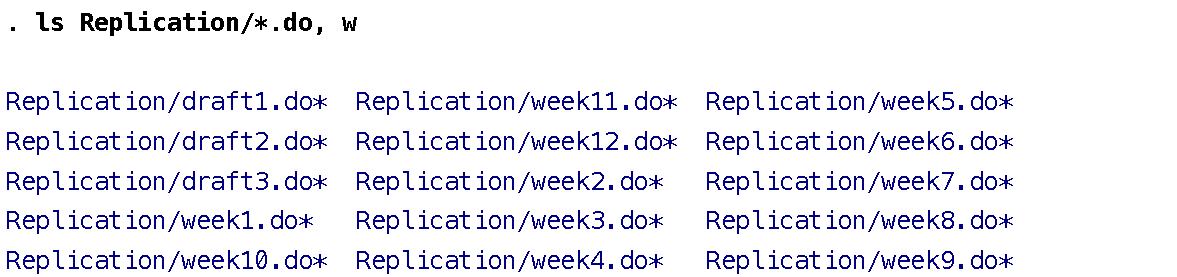
\includegraphics[scale=.5]{images/ls-replication}

	\caption{The contents of the \code folder.}%
    \label{fig:ls-replication}
\end{figure}

The \texttt{week*.do} files are used during our weekly sessions during the practice hour, and should be replicated at home as coursework. The \texttt{draft*.do} files provide template code for each stage of your research paper, from early to final draft.

To open the first weekly do-file in Stata, type \statacode{doedit code/week1}, which is the short form of the \statacode{doedit "code/week1.do"} command (the quotes around the folder path would be required if the path to \texttt{week1.do} contained spaces).} %
The file will open in the Stata do-file editor, in colored syntax display.


\paragraph{Color syntax}%
%
Stata lists most text in black. Default Stata commands are shown in dark blue, comments in green, numerical values in light blue and character strings in red. You can observe a sample of these colors by copy-pasting the following example code to a new do-file window:

\begin{docspec}
	* Load European Social Survey data.\\
	use data/ess2008, clear\\
	* Chi-squared test for gender and self-assessed health.\\
	tab gndr health if agea < 65, chi2
\end{docspec}

In this example, the first and third lines are comments, as indicated by their \texttt{*} prefix. The rest of the code executes two commands consecutively:

\begin{enumerate}
	\item %
  The \cmd{use} command opens the \texttt{ess2008} (\ess) dataset from the \data folder. This command works under the same assumptions as the \cmd{doedit} commands covered above. When successful, the \cmd{use} command does not necessarily produce any result, as shown here.%

	\item %
  The \cmd{tab}{tabulate} command uses the variable names \texttt{gndr} (gender) and \texttt{health} (self-assessed health status) as its arguments. The part of the command located after the comma is an option, \opt{chi2}{tab}, to add the result of a Chi-squared test to the cross-tabulation. This test is covered in Section~\ref{sec:chi2}.%
\end{enumerate}


\paragraph{Run one or more lines}%
%
Here.


% ========
% = HELP =
% ========


%
\section{Help}

Any professional who uses a computer has to rely on reading documentation and finding help. Similarly, quantitative methods cannot be learnt once and for all: the course will require that you frequently search for help, either within the course material or from additional online sources.


%
%
\subsection{Help for Stata}

Some of the most useful help resources will come from Stata itself, which comes with pretty good documentation. There is a also a wealth of short guides and detailed answers to hundreds of questions online. If you have to turn to Google, expect more random results and consider emailing us.


\paragraph{Stata \cmd{help}}%
%
Stata comes with its own internal documentation through the \cmd{help} command. The help pages cover the precise syntax and full options of all default commands and also document other aspects of how Stata syntax works. All pages can also be accessed online.\footnote{\url{http://www.stata.com/help.cgi?help}}

Getting to use the Stata help pages is a course objective in itself: even experienced Stata users use help pages on a daily basis. The details on each option and the final examples are often very useful in learning to use some commands efficiently.


\paragraph{Stata Press}%
%
Stata Press also publishes a series of manuals and handbooks that explore specific applications and more sophisticated uses of the software. Appropriate references for this course are the ``Getting Started'' manuals, which cover the same basic operations as this guide.\footnote{See \url{http://www.stata-press.com/}. The \emph{Stata Journal} is another publication that regularly describes new packages and user tips.} %%% TODO: add bib refs.


\paragraph{Online tutorials}%
%
An online search with the right keywords will lead you to online Stata tutorials published on websites and blogs. A selection of tutorials is available from the course website, but dozens more are floating around. One particularly interesting resource for beginners is the Stata video series by the LSE Methodology Institute.\footnote{\url{http://www.youtube.com/user/MethodologyLSE/videos?query=stata}} Stata also runs its own blog and video channel.\footnote{\url{http://blog.stata.com/2012/09/26/stata-youtube-channel-announced/}}


\paragraph{Online communities}%
%
Some services like Statalist\footnote{\url{http://stata.com/statalist/}} or Stackoverflow\footnote{\url{http://stackoverflow.com/questions/tagged/stata}} are particularly useful to find other Stata users who want to share questions and answers about the software.


\paragraph{Email assistance}%
%
The benefits of learning to search for documentation and help cannot be exaggerated, but if you are still stuck after getting through the course material, and in this case only, email your instructor(s) and ask your question as precisely as possible. If relevant, provide the code with which you are experiencing issues.


%
%
\subsection{Readings on statistics}

If you are looking for help on statistics, please first refer to the course readings listed in the course syllabus. Feinstein and Thomas’ \emph{Making History Count} (Cambridge University Press, 2002) and Moore \emph{et al.}'s \emph{Introduction to the Practice of Statistics} (W.H. Freeman, 6th ed., 2009) are the main handbooks for this course. Help on graphics and other topics can also be found in the additional readings.



%
% end
%